\documentclass[9pt]{article}

% --- Packing + layout ---
\usepackage{fancyhdr}
\usepackage[letterpaper,margin=0.3in,includehead,includefoot,headheight=14pt,headsep=6pt]{geometry}
\setlength{\columnsep}{0.15in}
\usepackage{microtype}
\usepackage{multicol}
\setlength{\parindent}{0pt}
\setlength{\parskip}{0pt}

% Tighten section spacing
\usepackage[compact,small]{titlesec}
\titlespacing*{\section}{0pt}{2pt}{1pt}
\titlespacing*{\subsection}{0pt}{2pt}{1pt}

% Tighten lists
\usepackage{enumitem}
\setlist{nosep,leftmargin=*}
\setlist[itemize]{noitemsep,topsep=0pt,parsep=0pt,partopsep=0pt,leftmargin=*}
\setlist[enumerate]{noitemsep,topsep=0pt,parsep=0pt,partopsep=0pt,leftmargin=*}

% Math spacing
\setlength{\abovedisplayskip}{2pt}
\setlength{\belowdisplayskip}{2pt}
\setlength{\abovedisplayshortskip}{1pt}
\setlength{\belowdisplayshortskip}{1pt}

% Math + links
\usepackage{amsmath,amssymb}
\usepackage[hidelinks]{hyperref}

% For including images
\usepackage{graphicx}
\usepackage{tikz}
\usetikzlibrary{calc}

% Callout boxes (kept for consistency even if unused)
\usepackage[most]{tcolorbox}
\tcbset{colback=white,colframe=black,boxrule=0.4pt,arc=2pt,left=6pt,right=6pt,top=4pt,bottom=4pt}
\newtcolorbox{notebox}{title=Note}
\newtcolorbox{solutionbox}{title=Solution}

% --- Fancy header/footer ---
\setlength{\headheight}{14pt}
\pagestyle{fancy}
\fancyhf{}
\fancyhead[L]{\textbf{Core Assessment 2 2026-01-27}}
\fancyfoot[C]{\thepage}
\renewcommand{\headrulewidth}{0.4pt}
\fancypagestyle{plain}{%
  \fancyhf{}
  \fancyhead[L]{\textbf{Core Assessment 2}}
  \fancyfoot[C]{\thepage}
  \renewcommand{\headrulewidth}{0.4pt}
}

\begin{document}

% --- Content ---
The following problems are a pool of items for your \textbf{C2 Assessment — Sets}. \textbf{Please practice these problems!}
\begin{multicols}{3}

\section*{A Venn Diagram}

\begin{center}
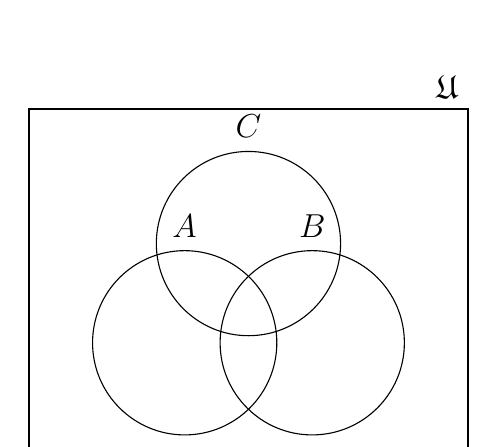
\begin{tikzpicture}[scale=0.9]
    % Draw rectangle around circles with label
    \draw[thick] (-2.2,-1.6) rectangle (4.0,3.3) node[above left]{\large $\mathfrak{U}$};
    % circle radius
    \def\rad{1.3}
    % circle centers
    \coordinate (A) at (0,0);
    \coordinate (B) at (1.8,0);
    \coordinate (C) at (0.9,1.4);
    % circles
    \draw (A) circle (\rad);
    \draw (B) circle (\rad);
    \draw (C) circle (\rad);
    % labels
    \node at ($(A)+(0,\rad+0.35)$) {\large $A$};
    \node at ($(B)+(0,\rad+0.35)$) {\large $B$};
    \node at ($(C)+(0,\rad+0.35)$) {\large $C$};
\end{tikzpicture}
\end{center}

Shade the regions of the Venn diagram for which each of the following expressions evaluates to True:

\begin{enumerate}[label=\arabic*., start=1]
    \item $(x \in A \cup B)\to  x \in C$
    \item $(x \in A\to x \in B)\land x\in C$
    \item $x \in A \setminus B \lor x \in C$
    \item $x \in A \leftrightarrow x\in B \setminus C$
    \item $x \in \overline{A} \lor (x\in B \cup C)$
\end{enumerate}

\vfill

\section*{B Reading Plots}


% --- Insert images ---

\includegraphics[width=\linewidth]{images/set_plot1.jpg}

\medskip

\includegraphics[width=\linewidth]{images/set_plot2.jpg}

\medskip

\includegraphics[width=\linewidth]{images/set_plot3.jpg}

\medskip

\includegraphics[width=\linewidth]{images/set_plot4.jpg}

\medskip

\includegraphics[width=\linewidth]{images/set_plot5.jpg}

\columnbreak

For the given plots above, mark each of the following expressions as true or false:

\begin{enumerate}[label=\alph*)]
    \item $\forall x \exists y,\,(x,y)\in S$
    \item $\forall x \exists !y,\,(x,y)\in S$
    \item $\forall y \exists x,\,(x,y)\in S$
    \item $\forall y \exists !x,\,(x,y)\in S$
    \item $\exists x \forall y,\,(x,y)\in S$
    \item $\exists !x \forall y,\,(x,y)\in S$
    \item $\exists y \forall x,\,(x,y)\in S$
    \item $\exists !y \forall x,\,(x,y)\in S$
\end{enumerate}

\section*{C. Test coverage with closure properties}

Let $A=\{0,1,2,3\}$. Suppose we are testing a function on inputs from $A \times A$.  
Let $B \subseteq A \times A$ be the set of failing inputs.  
In each of the following cases, assume $B$ has the stated closure property.  
Determine how many tests are needed to guarantee correctness.

\begin{enumerate}[label=\arabic*., start=1]

\item 
If $(a,b)\in B$ with $a \geq 1$, then $(a-1,b)\in B$.

\item
If $(a,b)\in B$ with $a,b \geq 1$, then $(a-1,b-1)\in B$.

\item
If $(a,b)\in B$ with $a\geq 1$, then $(a-1,b)\in B$ and if $b\geq 1$, then $(a,b-1)\in B$.

\item
If $(a,b)\in B$ with $a \geq 2$, then either $(a-1,b)\in B$ or $(a-2,b)\in B$.

\end{enumerate}
\vfill
\section*{D. Breakfast Counting Problems}

You are ordering breakfast. The choices are:
\begin{align*}
O=&\{\text{onion},\ \text{olives},\ \text{ham}\}\\
T=&\{\text{wheat},\ \text{white}\}\\
M=&\{\text{sausage},\ \text{bacon},\ \text{fruit}\}
\end{align*}
You may have any subset of $O$ as omelet toppings, choose one toast from $T$, and choose one meat from $M$. For the following questions, express your solution as a product, no simplification is necessary.

\begin{enumerate}[label=\arabic*., start=1]

\item  
How many possible orders if an English muffin is added to the toast options?

\item  
How many possible orders if instead of toast you can pick two meats, and doubling up meats is allowed?

\item  
How many possible orders if instead of toast you can pick two meats, but doubling up is \emph{not} allowed?

\item  
How many possible orders if green peppers are added to the omelet toppings?

\item  
How many possible orders if breakfast also comes with either coffee or orange juice (or both)?

\end{enumerate}

\end{multicols}
\newpage
\section*{E. Reading Tables}

The tables below show the outcomes of two different treatments, broken down by two groups of patients.  

\begin{itemize}
  \item Each cell shows a \textbf{fraction} (number of successes out of the total patients) and the corresponding \textbf{percentage} (success rate).
  \item The \textbf{Row Total} column shows the combined results of both treatments within that group.
  \item The \textbf{Overall} row shows the combined results across all groups.
  \item Pay attention: in each group, one treatment looks better, but when groups are combined, the overall result may tell a different story.
\end{itemize}

\begin{enumerate}
\item
{\renewcommand{\arraystretch}{1.3}
\begin{tabular}{lccc}
\hline
Group & Treatment A & Treatment B & Row Total \\
\hline
Group1 & 30\% (30/100) & 40\% (400/1000) & 430/1100 (39.1\%) \\
Group2 & 80\% (800/1000) & 90\% (90/100) & 890/1100 (80.9\%) \\
\hline
Overall & 75.5\% (830/1100) & 44.5\% (490/1100) & 1320/2200 (60.0\%) \\
\hline
\end{tabular}}


\vspace{1cm}
\item
{\renewcommand{\arraystretch}{1.3}
\begin{tabular}{lccc}
\hline
Group & Treatment A & Treatment B & Row Total \\
\hline
Group1 & 100\% (10/10) & 95\% (950/1000) & 960/1010 (95.0\%) \\
Group2 & 20\% (200/1000) & 30\% (30/100) & 230/1100 (20.9\%) \\
\hline
Overall & 20.8\% (210/1010) & 89.1\% (980/1100) & 1190/2110 (56.4\%) \\
\hline
\end{tabular}}
\vspace{1cm}
\item
{\renewcommand{\arraystretch}{1.3}
\begin{tabular}{lccc}
\hline
Group & Treatment A & Treatment B & Row Total \\
\hline
Group1 & 90\% (9/10) & 85\% (85/100) & 94/110 (85.5\%) \\
Group2 & 25\% (25/100) & 40\% (4/10) & 29/110 (26.4\%) \\
\hline
Overall & 30.9\% (34/110) & 80.9\% (89/110) & 123/220 (55.9\%) \\
\hline
\end{tabular}}
\vspace{1cm}
\item
{\renewcommand{\arraystretch}{1.3}
\begin{tabular}{lccc}
\hline
Group & Treatment A & Treatment B & Row Total \\
\hline
Group1 & 30\% (300/1000) & 20\% (20/100) & 320/1100 (29.1\%) \\
Group2 & 70\% (70/100) & 60\% (600/1000) & 670/1100 (60.9\%) \\
\hline
Overall & 33.6\% (370/1100) & 56.4\% (620/1100) & 990/2200 (45.0\%) \\
\hline
\end{tabular}}
\vspace{1cm}
\item
{\renewcommand{\arraystretch}{1.3}
\begin{tabular}{lccc}
\hline
Group & Treatment A & Treatment B & Row Total \\
\hline
Group1 & 70\% (700/1000) & 80\% (80/100) & 780/1100 (70.9\%) \\
Group2 & 40\% (40/100) & 50\% (500/1000) & 540/1100 (49.1\%) \\
\hline
Overall & 67.3\% (740/1100) & 52.7\% (580/1100) & 1320/2200 (60.0\%) \\
\hline
\end{tabular}}
\end{enumerate}
\vspace{1cm}
\section*{Comprehension Questions}

\begin{enumerate}
  \item[(a)] how many people took part in this study in total?  
  \item[(b)] how many people were in group 1?  
  \item[(c)] how many people were in group 2?  
  \item[(d)] out of group 1, which treatment had a higher percentage of successfully treated patients?  
  \item[(e)] out of group 2, which treatment had a higher percentage of successfully treated patients?  
  \item[(f)] out of the two groups, which group had a higher percentage of successfully treated patients?  
  \item[(g)] out of the two treatments, which treatment had a higher percentage of successfully treated patients?
\end{enumerate}

\end{document}
